% ============================================================================
% Climate Economics and Stochastic IAMs with DEQNs
% Deep Learning for Solving and Estimating Dynamic Models
% Duration: ~75 minutes (~35 frames)
% ============================================================================

\documentclass[aspectratio=169,11pt]{beamer}

% ---------- Theme and colors ----------
\usecolortheme{dove}
\setbeamertemplate{navigation symbols}{}
\setbeamertemplate{footline}{%
  \hfill\usebeamerfont{page number in head/foot}%
  \usebeamercolor[fg]{normal text}%
  \insertframenumber\,/\,\inserttotalframenumber\kern1em\vskip4pt}
\setbeamerfont{frametitle}{size=\huge}

% ---------- Packages ----------
\usepackage[utf8]{inputenc}
\usepackage[T1]{fontenc}
\usepackage{amsmath,amssymb,amsfonts}
\usepackage{bm}
\usepackage{graphicx}
\graphicspath{{fig/}}
\usepackage{tikz}
\usetikzlibrary{shapes,arrows.meta,positioning,calc,fit,backgrounds,patterns,decorations.pathreplacing}
\usepackage{pgfplots}
\pgfplotsset{compat=1.18}
\usepackage{booktabs}
\usepackage{hyperref}
\usepackage{multicol}
\usepackage{xcolor}

% ---------- Custom colors ----------
\definecolor{uzhblue}{rgb}{0,0,0.5}
\definecolor{uzhgreylight}{RGB}{236,238,241}
\definecolor{uzhgreydark}{RGB}{81,86,94}
\definecolor{harvardcrimson}{RGB}{153,0,0}
\definecolor{unil@blue}{RGB}{0,140,204}
\definecolor{unil@black}{RGB}{35,31,32}
\definecolor{darkgreen}{RGB}{0,100,0}
\definecolor{darkred}{RGB}{139,0,0}
\definecolor{softblue}{RGB}{70,130,180}
\definecolor{softorange}{RGB}{230,159,0}
\definecolor{softgreen}{RGB}{0,158,115}

% ---------- Set beamer colors ----------
\setbeamercolor{frametitle}{bg=uzhgreylight, fg=uzhblue}
\setbeamercolor{title}{fg=uzhblue}
\setbeamercolor{structure}{fg=uzhblue}
\setbeamercolor{block title}{bg=unil@blue, fg=white}
\setbeamercolor{block body}{bg=uzhgreylight}
\setbeamercolor{block title alerted}{bg=darkred,fg=white}
\setbeamercolor{block body alerted}{bg=red!5}
\setbeamercolor{block title example}{bg=darkgreen,fg=white}
\setbeamercolor{block body example}{bg=green!5}
\setbeamercolor{item}{fg=unil@black}
\setbeamercolor{normal text}{fg=unil@black}

% ---------- Emphasis and hyperlinks ----------
\newcommand{\emphc}[1]{\textcolor{harvardcrimson}{#1}}
\hypersetup{colorlinks,linkcolor=harvardcrimson,urlcolor=harvardcrimson}

% ---------- Math commands ----------
\newcommand{\x}{\bm{x}}
\newcommand{\X}{\bm{X}}
\newcommand{\R}{\mathbb{R}}
\newcommand{\E}[1]{\mathbb{E}\!\left[#1\right]}
\newcommand{\nn}{\mathcal{N}_{\bm{\rho}}}
\DeclareMathOperator*{\argmin}{arg\,min}
\DeclareMathOperator*{\argmax}{arg\,max}
\DeclareMathOperator{\Var}{Var}

% ---------- Title ----------
\title[Deep Learning for Dynamic Economic Models]
{Deep Learning for Economics and Finance}
\subtitle{DICE, CDICE, the carbon cycle, temperature dynamics, deterministic baseline}
\author{Simon Scheidegger}
\institute[HEC Lausanne]{HEC, University of Lausanne}
\date{}

\begin{document}
% --- Exercise pause badge ---
\newcommand{\exercisepause}{%
  \tikz[baseline=(X.base)]{\node[fill=darkgreen!80!black, text=white,
  rounded corners=2pt, inner sep=3pt, font=\scriptsize\bfseries](X){PAUSE --- 5 min};}}


% ============================================================================
% SECTION 0: TITLE & ROADMAP
% ============================================================================

% --- Frame 1: Title ---
{\setbeamercolor{background canvas}{bg=uzhgreylight}
\begin{frame}
\titlepage
\vspace{-0.4cm}
\begin{center}
{\footnotesize Based on: Nordhaus (2017), Folini, Friedl, K\"ubler, Scheidegger (2025, \textit{Restud}),}\\[1pt]
{\footnotesize Friedl, K\"ubler, Scheidegger, Usui (2023)}\\[4pt]
{\footnotesize Readings: see \texttt{readings/links\_by\_lecture/lecture\_16.md}}\\[4pt]
{\footnotesize Materials: \url{https://github.com/sischei/Deep_Learning_for_Solving_And_Estimating_Dynamic_Economic_Models}}
\end{center}
\end{frame}
}

% --- Frame 2: Roadmap ---
\begin{frame}{Roadmap of This Lecture}
\begin{center}
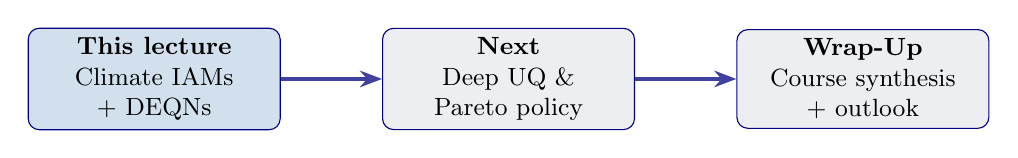
\begin{tikzpicture}[
    box/.style={rectangle, draw=uzhblue, fill=uzhgreylight, rounded corners=4pt,
                minimum width=3.2cm, minimum height=1.1cm, align=center, font=\small},
    arr/.style={-{Stealth[length=2.8mm]}, very thick, uzhblue!75}
]
\node[box, fill=softblue!25] (here) at (0,0) {\textbf{This lecture}\\Climate IAMs\\+ DEQNs};
\node[box] (next) at (4.5,0) {\textbf{Next}\\Deep UQ \&\\Pareto policy};
\node[box] (wrap) at (9,0) {\textbf{Wrap-Up}\\Course synthesis\\+ outlook};

\draw[arr] (here) -- (next);
\draw[arr] (next) -- (wrap);
\end{tikzpicture}
\end{center}

\vspace{0.3cm}
\textbf{This lecture}:
\begin{enumerate}
    \item Motivation: why climate economics?
    \item The DICE/CDICE climate model
    \item A stochastic IAM: full model and derivation
    \item Deep uncertainty quantification
\end{enumerate}
\end{frame}

% --- Learning objectives ---
\begin{frame}{Learning objectives}
\textbf{By the end of this lecture you should be able to:}
\begin{itemize}
  \item Derive climate-economic coupling equations from Lagrangian FOCs and envelope conditions
  \item Implement deterministic and stochastic IAMs with DEQNs handling nonstationary exogenous sequences
  \item Construct GP surrogates for SCC and welfare outputs via Bayesian active learning
  \item Compute global sensitivity decompositions (Sobol, Shapley) to identify parameter drivers of uncertainty
  \item Apply deep-UQ pipelines to quantify tail distributions and risk in long-horizon climate projections
\end{itemize}
\end{frame}


% ============================================================================
% SECTION I: MOTIVATION
% ============================================================================
\section{Motivation --- Why Climate Economics?}

% --- Frame 3: Section Divider ---
\begin{frame}{}
\vfill
\begin{center}
{\Huge \textcolor{uzhblue}{\textbf{Part I}}}\\[12pt]
{\LARGE Why Climate Economics?}
\end{center}
\vfill
\end{frame}

% --- Frame 4: Climate change as economic threat ---
\begin{frame}{Climate Change as an Economic Threat}
\begin{columns}[T]
\column{0.48\textwidth}
\includegraphics[width=\linewidth]{global-warming.png}
{\footnotesize Observed global warming motivates the IAM feedback loop below.}

\column{0.50\textwidth}
\begin{itemize}
    \item Global warming is a growing threat to economic well-being.
    \item Tipping points place us in catastrophic danger.
    \item Impacts current and future generations in different regions very differently.
    \item Recent overviews: Dietz (2024), van der Ploeg and Rezai (2026), Fernandez-Villaverde, Gillingham, Scheidegger (2025).
\end{itemize}
\end{columns}
\end{frame}

% --- Frame 5: Why IAMs ---
\begin{frame}{Why Integrated Assessment Models (IAMs)?}
\begin{block}{IAM logic}
Couple the \emphc{economy} (output, investment, abatement, welfare) with the \emphc{climate system}
(carbon concentrations, temperature, damages).
\end{block}

\vspace{0.05cm}
\begin{center}
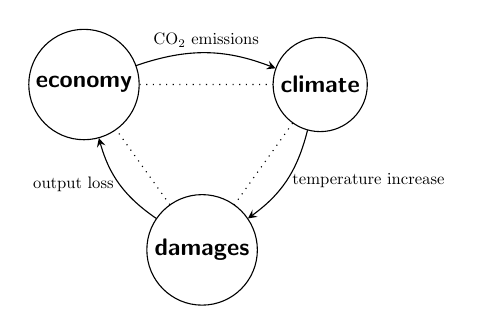
\begin{tikzpicture}[>=stealth, node distance=2cm, scale=0.60, transform shape]
    \tikzstyle{main node} = [circle, draw, minimum size=1.2cm, font=\sffamily\Large\bfseries]
    \node[main node] (economy) at (0,0) {economy};
    \node[main node] (climate) at (5,0) {climate};
    \node[main node] (damages) at (2.5,-3.5) {damages};
    \draw[->] (economy) to[bend left=20] node[above] {CO$_2$ emissions} (climate);
    \draw[->] (climate) to[bend left=20] node[right] {temperature increase} (damages);
    \draw[->] (damages) to[bend left=20] node[left] {output loss} (economy);
    \draw[dotted] (economy) -- (climate) -- (damages) -- (economy);
\end{tikzpicture}
\end{center}

\textbf{Output of interest:} social cost of carbon (SCC), optimal tax paths, welfare decomposition.
\vspace{-0.05cm}
\end{frame}

% --- Frame 6: Social cost of carbon ---
\begin{frame}{The Social Cost of Carbon (SCC)}
\begin{block}{Definition}
SCC at time $t$: marginal welfare cost of one extra unit of emissions, converted to consumption units.
\end{block}

\vspace{0.2cm}
\[
\mathrm{SCC}_t = -\frac{\partial V_t / \partial E_t}{\partial V_t / \partial C_t}
\]

\begin{columns}[T]
\column{0.49\textwidth}
\textbf{High SCC when}
\begin{itemize}
    \item Damages are steep
    \item Climate response is strong
    \item Discounting is low
    \item Tipping risk is material
\end{itemize}

\column{0.49\textwidth}
\textbf{Policy interpretation}
\begin{itemize}
    \item Tax path for carbon pricing
    \item Benchmark for regulation / cap-and-trade
    \item Input to cost-benefit analysis
    \item Why uncertainty matters: SCC is a \emphc{distribution}
\end{itemize}
\end{columns}
\end{frame}

% --- Frame 7: Why computationally hard ---
\begin{frame}{Why This Is Computationally Hard}
\begin{columns}[T]
\column{0.55\textwidth}
\begin{itemize}
    \item \textbf{Nonstationarity}: TFP, population, emissions intensity, and forcing paths all change exogenously over time.
    \item \textbf{Coupled dynamics}: economy and climate interact in both directions.
    \item \textbf{Long horizon}: welfare effects unfold over 100--300 years.
    \item \textbf{Curse of dimensionality}: nonlinearities, tipping hazards, constraints.
\end{itemize}

\column{0.42\textwidth}
\includegraphics[width=0.88\linewidth]{cod.png}\\[4pt]
\includegraphics[width=0.88\linewidth]{examplefunc.pdf}
\end{columns}
\end{frame}

% --- Frame 8: Our contribution ---
\begin{frame}{Our Contribution}
\begin{itemize}
    \item \textcolor{blue}{\textbf{Generic global solution method}} to efficiently compute global solutions to stochastic IAMs that include economic and climate risks.
    \item \textcolor{blue}{\textbf{Perform global sensitivity analysis}} with respect to uncertain parameters most discussed in the literature.
\end{itemize}

\vspace{0.2cm}
\begin{enumerate}
    \item Exploit \textbf{deep equilibrium nets} (DEQNs) to alleviate the curse of dimensionality.
    \item Add model parameters as \textbf{pseudo-states} $\rightarrow$ solve the model only \emphc{once}.
    \item Construct \textbf{surrogate models} for the SCC (and other QoIs) using \textbf{Gaussian Process regression} and \textbf{Bayesian active learning}.
\end{enumerate}
\end{frame}

% ============================================================================
% SECTION II: DICE/CDICE CLIMATE MODEL
% ============================================================================
\section{The DICE/CDICE Climate Model}

% --- Frame 9: Section Divider ---
\begin{frame}{}
\vfill
\begin{center}
{\Huge \textcolor{uzhblue}{\textbf{Part II}}}\\[12pt]
{\LARGE The DICE/CDICE Climate Model}
\end{center}
\vfill
\end{frame}

% --- Frame 10: DICE baseline ---
\begin{frame}{DICE Baseline: Minimal Global IAM}
\small
\begin{columns}[T]
\column{0.56\textwidth}
\textbf{State variables}
\begin{itemize}
    \item Economic stock: $K_t$
    \item Carbon stocks: $M_t^{\mathrm{AT}}, M_t^{\mathrm{UO}}, M_t^{\mathrm{LO}}$
    \item Temperature states: $T_t^{\mathrm{AT}}, T_t^{\mathrm{OC}}$
    \item Exogenous trends: population $L_t$, TFP $A_t$, emissions intensity $\sigma_t$
\end{itemize}

\textbf{Controls}
\begin{itemize}
    \item Savings / investment share $s_t$
    \item Abatement rate $\mu_t$
\end{itemize}

\column{0.41\textwidth}
\begin{exampleblock}{Why DICE is influential}
\begin{itemize}
    \item Transparent
    \item Fast to evaluate
    \item Policy-facing
    \item Benchmark for extensions
\end{itemize}
\end{exampleblock}
\end{columns}

\vspace{0.2cm}
\begin{alertblock}{Challenge}
Fast is useful, but only if the climate module is calibrated consistently with climate science.
\end{alertblock}
\end{frame}

% --- Frame 11: Carbon cycle ---
\begin{frame}{Carbon Cycle (3-Box Model)}
\small
\begin{itemize}
    \item DICE-2016 models the carbon cycle via three carbon reservoirs:
    \begin{itemize}
        \item Atmosphere (AT), Upper ocean (UO), Lower ocean (LO)
    \end{itemize}
    \item Aggregate distribution of carbon: $M_t = (M_{\mathrm{AT},t}, M_{\mathrm{UO},t}, M_{\mathrm{LO},t})^T$
\end{itemize}

\vspace{0.2cm}
\textbf{Carbon concentrations evolve as a linear dynamic system:}
\[
M_{t+1} = (I + \Delta_t \cdot B) \cdot M_t + \Delta_t \cdot E_t
\]

\begin{itemize}
    \item Carbon emissions (economic activity + exogenous source): $E_t = E_{\mathrm{ind},t} + E_{\mathrm{Land}}$
    \item Industrial emissions: $E_{\mathrm{ind},t} = (1-\mu_t)\sigma_t K_t^{\alpha}(A_t L_t)^{1-\alpha}$
    \item $B$ is the transfer matrix governing exchange rates between reservoirs
\end{itemize}
\end{frame}

% --- Finger Exercise: Carbon Cycle ---
\begin{frame}{\exercisepause{} Finger Exercise: One-Step Carbon Cycle}
\begin{exampleblock}{Exercise}
The simplified carbon cycle has atmospheric CO$_2$ evolving as:
\[
M_{\text{AT}}^{t+1} = E_t + \phi_{11}\, M_{\text{AT}}^{t} + \phi_{21}\, M_{\text{UP}}^{t},
\]
where $\phi_{11} = 0.912$, $\phi_{21} = 0.0444$, and $M_{\text{UP}}^t$ (upper ocean) is given.
\begin{enumerate}
    \item With $M_{\text{AT}}^{2020} = 851$ GtC, $M_{\text{UP}}^{2020} = 628$ GtC, and emissions $E_{2020} = 10$ GtC/yr (over a 5-year step: $E = 50$ GtC): compute $M_{\text{AT}}^{2025}$.
    \item If emissions doubled to $E = 100$ GtC, what would $M_{\text{AT}}^{2025}$ be?
    \item By how many GtC does doubling emissions increase atmospheric CO$_2$?
\end{enumerate}
\end{exampleblock}
\end{frame}

\begin{frame}{Solution: One-Step Carbon Cycle}
\begin{block}{Answer}
\begin{enumerate}
    \item $M_{\text{AT}}^{2025} = 50 + 0.912 \times 851 + 0.0444 \times 628 = 50 + 776.1 + 27.9 = 854.0$ GtC.
    \item $M_{\text{AT}}^{2025} = 100 + 776.1 + 27.9 = 904.0$ GtC.
    \item Doubling emissions adds $904.0 - 854.0 = 50$ GtC---exactly the extra emissions.  The carbon cycle is \emphc{linear} in emissions (at one-step horizon), so the effect is additive.
\end{enumerate}
\end{block}
\end{frame}

% --- Frame 12: Temperature dynamics ---
\begin{frame}{Temperature Dynamics (2-Box Model)}
\small
The two-layer energy balance model in DICE-2016:
\begin{align*}
    T^{\mathrm{AT}}_{t+1} &= T^{\mathrm{AT}}_{t} + \Delta_t \cdot c_{1} \left(F_{t} - \lambda T^{\mathrm{AT}}_{t} - c_{3}\left(T^{\mathrm{AT}}_{t} - T^{\mathrm{OC}}_{t}\right)\right) \\
    T^{\mathrm{OC}}_{t+1} &= T^{\mathrm{OC}}_{t} + \Delta_t \cdot c_{4} \left(T^{\mathrm{AT}}_{t} - T^{\mathrm{OC}}_{t}\right)
\end{align*}

\textbf{Radiative forcing:}
\[
    F_{t} = F_{\mathrm{2\times CO_2}} \frac{\log(M^{\mathrm{AT}}_{t}/M^{\mathrm{AT}}_{\mathrm{PI}})}{\log(2)} + F^{\mathrm{EX}}_{t}
\]

\begin{alertblock}{Key parameters}
$\lambda = F_{\mathrm{2\times CO_2}}/\Delta T_{\mathrm{AT},\times 2}$ where $\Delta T_{\mathrm{AT},\times 2}$ is the \emphc{equilibrium climate sensitivity} (ECS) --- the long-run warming from CO$_2$ doubling. $M^{\mathrm{AT}}_{\mathrm{PI}}$ is the preindustrial atmospheric CO$_2$ stock.
\end{alertblock}
\end{frame}

% --- Frame 13: Damage functions ---
\begin{frame}{Damage Functions}
\footnotesize
\begin{columns}[T]
\column{0.38\textwidth}
\includegraphics[width=0.88\linewidth]{damage.png}
{\scriptsize Damage fraction $\Omega(T)$: the share of gross output lost at warming $T$. Increasing in $T$.}

\column{0.60\textwidth}
\textbf{Nordhaus (2008):}
\[
\Omega^N(T_{\mathrm{AT}}) = \pi_1 T_{\mathrm{AT}} + \pi_2 T_{\mathrm{AT}}^{2}
\]

\textbf{Weitzman (2012) --- with tipping:}
\[
\Omega^W(T_{\mathrm{AT}}) = 1 - \frac{1}{1 + \left(\frac{1}{\psi_1} T_{\mathrm{AT}}\right)^{2} + \left(\frac{1}{2\, TP} T_{\mathrm{AT}}\right)^{6.754}}
\]
\end{columns}

\vspace{0.2cm}
\begin{itemize}
    \item Degree of convexity is of key importance in determining the optimal taxes [Weitzman 2012].
    \item Tipping points: losing the Amazon rain forest, faster onset of El Ni\~no, reversal of the Gulf Stream, etc.
\end{itemize}
\end{frame}

% --- Frame 14: Why recalibrate ---
\begin{frame}{Why Recalibrate? $\rightarrow$ CDICE}
\small
\begin{itemize}
    \item Climate emulators must reproduce benchmark behavior from climate science model archives (CMIP).
    \item Earlier critiques highlighted major discrepancies for common IAM calibrations.
    \item Folini et al.\ show that the \emphc{functional form can remain simple}, but parameters require systematic calibration.
\end{itemize}

\vspace{0.2cm}
\begin{center}
\includegraphics[width=0.88\textwidth]{CDICE-vs-DICE.png}
\end{center}
{\footnotesize CDICE recalibrates the reduced-form climate emulator to climate-science benchmarks.}
\end{frame}

% --- Frame 15: Four-test framework ---
\begin{frame}{Four-Test Framework (Folini et al., 2025)}
\scriptsize
\begin{center}
\begin{tabular}{lll}
\toprule
\textbf{Test} & \textbf{Targets} & \textbf{Use} \\
\midrule
1. Carbon pulse (100 GtC) & Atmospheric retention path & Calibrate carbon cycle \\
2. 4$\times$CO$_2$ step & Temperature impulse response & Calibrate temperature block \\
3. 1\% CO$_2$/year & Transient climate response (TCR) & Out-of-sample validation \\
4. Historical + RCP & Realistic forcing paths & End-to-end validation \\
\bottomrule
\end{tabular}
\end{center}

\vspace{0.2cm}
\begin{columns}[T]
\column{0.48\textwidth}
\includegraphics[width=\linewidth]{CCBM_100GtC_Puls.png}
{\footnotesize Carbon-pulse response.}

\column{0.48\textwidth}
\includegraphics[width=\linewidth]{TempBM_4xCO2_on_PI.png}
{\footnotesize Temperature response to a $4\times$CO$_2$ forcing step.}
\end{columns}
\end{frame}

% --- Frame 16: ECS uncertainty ---
\begin{frame}{Equilibrium Climate Sensitivity (ECS) --- A Key Uncertainty}
\begin{center}
\includegraphics[width=0.50\textwidth]{knutti.png}
\end{center}

\vspace{-0.15cm}
\small
\begin{itemize}\setlength\itemsep{0pt}
    \item Roe and Baker (2007): $\mathrm{ECS} = \frac{\lambda_0}{1-f} F_{\mathrm{2\times CO_2}}$, $f \sim \mathcal{N}(\mu_f, S_f)$.
    \item Making ECS stochastic is a natural channel for Bayesian learning.
\end{itemize}
\end{frame}

% --- Frame 17: Transparent time step ---
\begin{frame}{Transparent Time-Step Formulation}
\small
A practical contribution in CDICE: expose the time-step scaling directly in equations.
\[
X_{t+\Delta t} = X_t + \Delta t \cdot f(X_t, u_t; \theta)
\]

\begin{itemize}
    \item Allows coherent annual, 5-year, or 10-year implementations within one generic formulation.
    \item Time discretization consistency improves transferability between classroom code, production code, and policy simulation horizons.
\end{itemize}

\vspace{0.2cm}
\textbf{Summary of climate module:}
\begin{center}
\small
\begin{tabular}{ll}
\toprule
\textbf{Climate states (5)} & $M_{\mathrm{AT}}, M_{\mathrm{UO}}, M_{\mathrm{LO}}, T^{\mathrm{AT}}, T^{\mathrm{OC}}$ \\
\textbf{Key parameters} & ECS ($\Delta T_{\mathrm{AT},\times 2}$), carbon transfer $B$, forcing $F_{\mathrm{2\times CO_2}}$ \\
\textbf{Uncertainty channels} & ECS, damage curvature, tipping \\
\bottomrule
\end{tabular}
\end{center}
\end{frame}

% ============================================================================
% SECTION III: STOCHASTIC IAM --- FULL MODEL & DERIVATION
% ============================================================================
\section{A Stochastic IAM --- Full Model and Derivation}

% --- Frame 18: Section Divider ---
\begin{frame}{}
\vfill
\begin{center}
{\Huge \textcolor{uzhblue}{\textbf{Part III}}}\\[12pt]
{\LARGE A Stochastic IAM --- Full Derivation}
\end{center}
\vfill
\end{frame}

% --- Frame 19: Planner's problem ---
\begin{frame}{The Planner's Problem --- Epstein-Zin Preferences}
\small
The planner maximizes normalized recursive utility (Epstein-Zin):
\[
V(\X_t)^{1-1/\psi}
  = \max_{C_{t},K_{t+1},\mu_{t}}\left\{(1-\beta^{\mathrm{EZ}}_t)\left( \frac{C_{t}}{L_{t}} \right)^{1-1/\psi}L_{t}
    +
    \beta^{\mathrm{EZ}}_t \mathbb{E}_{t}\left[V(\X_{t+1})^{1-\gamma}\right]^{\frac{1-1/\psi}{1-\gamma}}\right\}
\]
with $\beta^{\mathrm{EZ}}_t=\exp(-\rho\Delta_t)$.

subject to: budget constraint, capital accumulation, climate dynamics, learning dynamics.

\vspace{0.2cm}
\begin{columns}[T]
\column{0.49\textwidth}
\textbf{Preference parameters}
\begin{itemize}
    \item $\psi$: intertemporal elasticity of substitution (IES)
    \item $\gamma$: risk aversion
    \item $\rho$: rate of time preference
\end{itemize}

\column{0.49\textwidth}
\begin{alertblock}{Why Epstein-Zin?}
Separate risk aversion from intertemporal substitution --- crucial for long-run climate risk.
\end{alertblock}
\end{columns}
\end{frame}

% --- Frame 20: Full constraint set ---
\begin{frame}{Full Constraint Set (10 Equations)}
\resizebox{\linewidth}{!}{
  \begin{minipage}{1.2\linewidth}
\begin{align*}
  &\text{Budget:} &
    \bigl(1-\Omega(T_{\mathrm{AT},t}) - \Theta(\mu_t)\bigr) K_{t}^{\alpha}( A_{t}L_{t} )^{1-\alpha}
    - C_{t} - I_{t} &= 0 \\
  &\text{Capital:} &
    ( 1-\delta )K_{t} + I_{t} - K_{t+1} &= 0\\
  &\text{Abatement bound:} &
    1 - \mu_{t} &\geq 0  \\
  &\text{Carbon (AT):} &
    (1-\phi_{12})M_{\mathrm{AT},t}+\phi_{21}M_{\mathrm{UO},t}+(1-\mu_{t})\sigma_{t}K_{t}^{\alpha}( A_{t}L_{t} )^{1-\alpha} + E_{\mathrm{Land},t} - M_{\mathrm{AT},t+1} &= 0 \\
  &\text{Carbon (UO):} &
    \phi_{12}M_{\mathrm{AT},t}+(1-\phi_{21}-\phi_{23})M_{\mathrm{UO},t}+\phi_{32}M_{\mathrm{LO},t}
  - M_{\mathrm{UO},t+1} &= 0 \\
  &\text{Carbon (LO):} &
    \phi_{23}M_{\mathrm{UO},t}+(1-\phi_{32})M_{\mathrm{LO},t} -
    M_{\mathrm{LO},t+1} &= 0 \\
  &\text{Temp (AT):} &
    T_{\mathrm{AT},t} + \text{[forcing + feedback + shock]} - T_{\mathrm{AT},t+1} &= 0 \\
  &\text{Temp (OC):} &
    \varphi_{4}T_{\mathrm{AT},t}+(1-\varphi_{4})T_{\mathrm{OC},t}
    -  T_{\mathrm{OC},t+1} &= 0 \\
  &\text{Learning ($\mu_f$):} &
    \text{Bayesian posterior update} - \mu_{f,t+1} &= 0\\
  &\text{Learning ($S_f$):} &
    \text{Variance update} - S_{f,t+1} &= 0
\end{align*}
\end{minipage}
}

\vspace{2pt}
{\scriptsize\emphc{In this lecture's notebooks:} \texttt{02}/\texttt{03} solve the \emphc{8-equation CDICE core} (the first eight rows); the two Bayesian ECS-learning equations ($\mu_f, S_f$) are the Friedl et al.\ research extension, not implemented here.}
\end{frame}

% --- Frame 21: KEY SLIDE --- Nonstationarity and time as state ---
\begin{frame}{Nonstationarity and Time as a State Variable}
\begin{alertblock}{The key difference from the discrete-time lectures}
IAMs are \emphc{nonstationary}: $A_t$ (TFP), $L_t$ (population), $\sigma_t$ (carbon intensity), $E_{\mathrm{Land},t}$, $F^{\mathrm{EX}}_t$ all change exogenously over time.
\end{alertblock}

\vspace{0.2cm}
\begin{itemize}
    \item Unlike Brock-Mirman or stationary OLG, we \emphc{cannot} have a time-invariant policy function.
    \item \textbf{Solution:} add $t$ as an explicit state variable to the neural network input.
    \item For neural net stability, transform: $\tau = 1 - \exp(-\vartheta \cdot t) \in [0,1)$
    \item Normalize capital, consumption, investment by $A_t \times L_t$ to detrend what we can.
    \item Time captures what \emphc{remains nonstationary} after detrending.
\end{itemize}

\vspace{0.2cm}
\begin{exampleblock}{Practical implication}
The policy network is $\nn(\tau_t, \text{states}, \text{params})$ --- transformed time is an \emphc{input}, not just an index.
\end{exampleblock}
\end{frame}

% --- Frame 22: State space summary ---
\begin{frame}{State Space Summary}
\[
\X_t = \Big[\underbrace{k_t, M_{\mathrm{AT},t}, M_{\mathrm{UO},t}, M_{\mathrm{LO},t}, T^{\mathrm{AT}}_t, T^{\mathrm{OC}}_t, \mu_{f,t}, S_{f,t}, \emphc{\tau_t}}_{\text{9 endogenous/exogenous states}};\; \underbrace{\theta}_{\text{$N$ pseudo-state parameters}}\Big]
\]

\vspace{0.2cm}
\begin{center}
\textcolor{blue}{\textbf{Minimal model has a 9+$N$-dimensional state space.}}
\end{center}

\vspace{0.2cm}
\begin{columns}[T]
\column{0.49\textwidth}
\textbf{Pseudo-state parameters $\theta$}
\begin{itemize}
    \item $\rho$ (time preference)
    \item $\gamma$ (risk aversion)
    \item $\psi$ (IES)
    \item $\pi_2$ (damage curvature)
    \item $\mu_{f,0}, S_{f,0}$ (ECS prior)
    \item Carbon cycle parameters
\end{itemize}

\column{0.49\textwidth}
\textbf{Why pseudo-states?}
\begin{itemize}
    \item Solve the model \emphc{once} for all parameter combinations
    \item UQ becomes interpolation on the learned surrogate
    \item From earlier DEQN lectures: the same trick used for $\beta, \alpha$ in Brock-Mirman
\end{itemize}
\end{columns}
\end{frame}

% --- Frame 23: Lagrangian ---
\begin{frame}{Derivation: The Lagrangian}
\small
Write the Lagrangian with multipliers ($\lambda$ for budget, $\xi$ for capital, $\eta$ for abatement):

\resizebox{0.95\linewidth}{!}{
  \begin{minipage}{\linewidth}
\begin{align*}
\mathcal{L} &= V(\X_t)^{1-1/\psi} \\
 &\quad + \lambda_t \Big[\bigl(1-\Omega(T_{\mathrm{AT},t}) - \Theta(\mu_t)\bigr) K_t^\alpha (A_t L_t)^{1-\alpha} - C_t - I_t\Big] \\
 &\quad + \xi_t \Big[(1-\delta)K_t + I_t - K_{t+1}\Big] \\
 &\quad + \eta_t \Big[1 - \mu_t\Big] \\
 &\quad + \text{[multipliers for carbon cycle, temperature, learning dynamics]}
\end{align*}
\end{minipage}
}

\vspace{0.2cm}
\textbf{Control variables:} $C_t$, $K_{t+1}$, $\mu_t$

\textbf{Strategy:} Take FOCs $\rightarrow$ use envelope theorem $\rightarrow$ derive Euler equations
\end{frame}

% --- Frame 24: FOCs ---
\begin{frame}{Derivation: First-Order Conditions}
\small
\textbf{w.r.t.\ $C_t$} (marginal utility = shadow price of budget):
\[
\frac{\partial V^{1-1/\psi}}{\partial C_t} = \lambda_t
\]

\textbf{w.r.t.\ $K_{t+1}$} (intertemporal trade-off):
\[
\xi_t = e^{-\rho} \frac{\partial}{\partial K_{t+1}} \mathbb{E}_t\!\left[V(\X_{t+1})^{1-\gamma}\right]^{\frac{1-1/\psi}{1-\gamma}}
\]

\textbf{w.r.t.\ $\mu_t$} (marginal abatement cost = marginal emission damage):
\[
\lambda_t \frac{\partial \Theta}{\partial \mu_t} K_t^\alpha (A_t L_t)^{1-\alpha} = \eta_t + \text{[shadow value of reduced emissions]}
\]

\vspace{0.2cm}
\begin{alertblock}{Problem}
Cannot compute $\partial V / \partial(\text{state}_{t+1})$ analytically $\rightarrow$ need the \emphc{envelope theorem}.
\end{alertblock}
\end{frame}

% --- Frame 25: Envelope theorem ---
\begin{frame}{Derivation: Envelope Theorem}
\small
The envelope theorem gives us derivatives of the value function w.r.t.\ \emphc{current} states:
\[
\frac{\partial V(\X_t)^{1-1/\psi}}{\partial k_t} = \lambda_t \cdot \alpha \bigl(1-\Omega(T_{\mathrm{AT},t}) - \Theta(\mu_t)\bigr) k_t^{\alpha-1}(A_t L_t)^{1-\alpha} + \xi_t \cdot (1-\delta)
\]
\[
\frac{\partial V(\X_t)^{1-1/\psi}}{\partial M_{\mathrm{AT},t}} = \text{[shadow value of atmospheric carbon]}
\]
\[
\frac{\partial V(\X_t)^{1-1/\psi}}{\partial T^{\mathrm{AT}}_t} = \text{[shadow value of temperature]}
\]

\vspace{0.2cm}
\textbf{Strategy:}
\begin{enumerate}
    \item Get $\partial V / \partial(\text{state}_t)$ from envelope
    \item Shift forward one period: $\partial V / \partial(\text{state}_{t+1})$
    \item Substitute back into FOCs to obtain \emphc{Euler equations}
\end{enumerate}
\end{frame}

% --- Frame 26: Euler equations ---
\begin{frame}{Derivation: Euler Equations}
\small
\textbf{Capital Euler equation:}
\[
1 = e^{-\rho}\, \mathbb{E}_t\!\left[\left(\frac{V_{t+1}}{(\mathbb{E}_t[V_{t+1}^{1-\gamma}])^{1/(1-\gamma)}}\right)^{1/\psi - \gamma} \cdot \frac{(C_{t+1}/L_{t+1})^{-1/\psi}}{(C_t/L_t)^{-1/\psi}} \cdot R_{t+1}^K\right]
\]
where $R_{t+1}^K$ is the return on capital including climate damages.

\vspace{0.2cm}
\textbf{SCC as shadow price of atmospheric carbon:}
\[
\mathrm{SCC}_t = -\frac{\partial V_t / \partial M_{\mathrm{AT},t}}{\partial V_t / \partial C_t}
\]
Captures the present-value welfare cost of one extra unit of atmospheric carbon.

\vspace{0.2cm}
\begin{exampleblock}{Abatement optimality}
At the optimum: marginal abatement cost $=$ carbon tax $=$ SCC (in the planner's problem).
\end{exampleblock}
\end{frame}

% --- Frame 27: Bayesian learning ---
\begin{frame}{Bayesian Learning Mechanics (literature)}
\small
Temperature evolves with uncertain climate feedback $\tilde{f}_{t+1} \sim \mathcal{N}(\mu_{f,t}, S_{f,t})$:
\[
T^{\mathrm{AT}}_{t+1} = \ldots + \varphi_{1C}\tilde{f}_{t+1} T^{\mathrm{AT}}_t + \tilde{\epsilon}_{T,t+1}
\]

\textbf{Gaussian conjugate posterior updates:}
\begin{align*}
\mu_{f,t+1} &= \frac{S_{\epsilon_T} \mu_{f,t} + \varphi_{1C} T^{\mathrm{AT}}_t \left(\varphi_{1C} T^{\mathrm{AT}}_t \tilde{f}_{t+1} + \tilde{\epsilon}_{T,t+1}\right) S_{f,t}}{S_{\epsilon_T} + \left(\varphi_{1C} T^{\mathrm{AT}}_t\right)^2 S_{f,t}} \\[4pt]
S_{f,t+1} &= \frac{S_{\epsilon_T} \cdot S_{f,t}}{S_{\epsilon_T} + \left(\varphi_{1C} T^{\mathrm{AT}}_t\right)^2 S_{f,t}}
\end{align*}

\begin{itemize}
    \item Agent observes shock realizations at the beginning of each period.
    \item Learning shifts optimal near-term abatement: \emphc{insurance motive today} vs.\ \emphc{information value tomorrow}.
\end{itemize}
\end{frame}

% --- Frame 28: From Euler to DEQN loss ---
\begin{frame}{From Euler Equations $\rightarrow$ DEQN Loss}
\begin{columns}[T]
\column{0.55\textwidth}
\small
Each equilibrium condition becomes a \emphc{residual}:
\[
G_i(\x, \nn) = 0 \quad \forall i
\]

\textbf{Loss function:}
\[
\ell_{\bm{\rho}} = \frac{1}{N} \sum_{\x_t} \sum_i G_i(\x_t, \nn)^2
\]

\begin{itemize}\setlength\itemsep{0pt}
    \item No labeled data needed
    \item $\nn$ simulates the path itself
    \item Train with SGD (Adam)
\end{itemize}

\column{0.40\textwidth}
\begin{center}
\includegraphics[width=\linewidth,height=0.55\textheight,keepaspectratio]{nn.png}
\end{center}
\end{columns}
\end{frame}

% --- Frame 29: Architecture details ---
\begin{frame}{DEQN Architecture for the Stochastic IAM}
\begin{columns}[T]
\column{0.52\textwidth}
\small
\begin{tabular}{ll}
\toprule
\textbf{Component} & \textbf{Specification} \\
\midrule
Hidden layers & 2 \\
Nodes per layer & 512 (1024 in production) \\
Activation & relu \\
Optimizer & Adam, $\alpha = 5\times10^{-5}$ \\
Batch size & 512 \\
Inputs & 9 + $N$ (states + pseudo) \\
Outputs & $k', \mu$, multipliers \\
\bottomrule
\end{tabular}

\vspace{0.15cm}
\textbf{Training workflow:}
\begin{enumerate}\setlength\itemsep{0pt}
    \item Simulate path with $\nn$
    \item Evaluate residuals on path
    \item Gradient descent on loss
    \item Mix broad \& endogenous sampling
\end{enumerate}

\column{0.45\textwidth}
\begin{center}
\includegraphics[width=0.85\linewidth]{cost_function.png}\\[2pt]
{\footnotesize Training loss convergence}
\end{center}
\end{columns}
\end{frame}

% --- Frame 29b: EZ + iid weather formulation (Friedl et al., literature/preview; no notebook in this lecture) ---
\begin{frame}{Epstein--Zin + i.i.d.\ weather (literature): model ingredients}
\small
\begin{alertblock}{Literature / preview --- not a notebook in this lecture}
\footnotesize The Epstein--Zin $+$ i.i.d.-weather formulation in the next four slides follows Friedl et al.\ (2023) and is shown as an advanced target. This lecture's stochastic notebook (\texttt{03}) implements the simpler \emphc{CRRA $+$ AR(1)} version (Cai--Lontzek spirit); EZ with tipping risk returns in the next lecture.
\end{alertblock}
\textbf{State (8-D):} $\X_t = [k_t, M_{\mathrm{AT},t}, M_{\mathrm{UO},t}, M_{\mathrm{LO},t}, T^{\mathrm{AT}}_t, T^{\mathrm{OC}}_t, \tau_t, w_t]$
\begin{itemize}\setlength\itemsep{0pt}
    \item $\tau_t = 1 - e^{-\vartheta t}$: time transform (handles nonstationarity).
    \item $w_t \sim \mathcal{N}(0,\sigma_w^2)$, iid: weather shock entering productivity and emissions intensity.
\end{itemize}

\textbf{Network (single):} $\nn : \X_t \mapsto (k', \hat\lambda, \mu, \nu^{\!AT}, \nu^{\!UO}, \nu^{\!LO}, \eta^{\!AT}, \eta^{\!OC}, V) \in \mathbb{R}^9$.

\textbf{Calibration:} $\psi = 0.69$ (IES), $\gamma = 10$ (RA), $\sigma_w = 0.01$, 5-node Gauss--Hermite over $w'$.

\vspace{0.15cm}
\begin{exampleblock}{Why a \emphc{single} 9-output network (Friedl style)?}
Shadow values $\nu, \eta$ are network outputs, not derivatives of $V$. This gives the optimizer direct gradient signal on every multiplier instead of forcing it through second derivatives of $V$ --- crucial when $V$ is itself being learned.
\end{exampleblock}
\end{frame}

% --- Frame 29c: The 9-residual EZ loss with v_+/v normalization ---
\begin{frame}{Epstein--Zin (literature): the 9-residual loss}
\footnotesize
With $\hat\beta = e^{-\rho}$, $e_1 = \frac{1-\gamma}{1-1/\psi}$, $e_2 = \frac{\gamma - 1/\psi}{1-\gamma}$, $e_3 = \frac{1/\psi - \gamma}{1-1/\psi}$:

\textbf{Capital Euler (eq 1):}
\[
e^{(g^{\!A}+g^{\!L})\Delta t}\,\hat\lambda_t \;=\; \hat\beta\,\big(\mathbb{E}_t[(V_+/V)^{e_1}]\big)^{e_2}\,\mathbb{E}_t\!\left[(V_+/V)^{e_3}\,v_{k,+}\right]
\]

\textbf{Budget (eq 2), KKT-$\mu$ (eq 3, Fischer–Burmeister, no expectation).}

\textbf{Envelope conditions on $T^{\!AT}, M^{\!AT}, M^{\!UO}, M^{\!LO}, T^{\!OC}$ (eq 4–8):}
\[
\eta^{\!AT}_t = \hat\beta\,(\mathbb{E}_t[(V_+/V)^{e_1}])^{e_2}\,\mathbb{E}_t[(V_+/V)^{e_3}\,v_{T^{\!AT}\!,+}], \quad \text{etc.}
\]

\textbf{EZ Bellman (eq 9, Bansal–Yaron normalized):}
\[
V_t^{1-1/\psi} = (1-\hat\beta)\,c_t^{1-1/\psi} + \hat\beta\,\big(\underbrace{\mathbb{E}_t[V_+^{1-\gamma}]}_{\textbf{not frozen}}\big)^{\!\frac{1-1/\psi}{1-\gamma}}
\]

\textbf{Loss:} $\mathcal{L}(\theta) = \frac{1}{9}\sum_{i=1}^{9}\mathbb{E}_{\X\sim\pi_\theta}[G_i(\X;\theta)^2]$ \quad (equal-weighted MSE).

\begin{alertblock}{$v_{t+1}/v_t$ normalization}
We never evaluate $V_+^{e_3}$ directly ($e_3 \approx 19$ at $\gamma=10$ blows up float32). Form ratios $V_+/V$ first, then take the power --- numerator and denominator stay $\mathcal{O}(1)$.
\end{alertblock}
\end{frame}

% --- Frame 29d: The freezing trick (stop_gradient on EZ corrections) ---
\begin{frame}{Freezing trick (literature): \texttt{stop\_gradient} on EZ corrections}
\footnotesize
\textbf{Pathology.} At $\gamma = 10$, $\psi = 0.69$ $\Rightarrow$ $e_3 \approx 19$. A 1\% spread in $V_+$ across GH nodes becomes a 19\% spread in $(V_+/V)^{e_3}$. The optimizer ``discovers'' it can shrink the FOC residual by moving $V$ --- but $V$ is also pinned by the Bellman equation (eq 9). The two forces fight, training oscillates.

\textbf{Fix.} Wrap every EZ correction in \texttt{tf.stop\_gradient}:
\begin{center}
\texttt{ez\_corr = tf.stop\_gradient(tf.pow(V\_n / V, e3))}
\end{center}
Forward pass keeps $\Phi = (V_+/V)^{e_3}$; backward pass treats $\Phi$ as a per-state \emphc{constant}.

\textbf{Fixed-point view.} Each Adam step is one iteration of:
\begin{enumerate}\setlength\itemsep{0pt}
    \item Evaluate $\Phi$ at current $\theta$ \emph{(frozen for backprop)}.
    \item FOC residuals (eq 1, 4--8) train $\mu, \lambda, \nu, \eta$ against frozen $\Phi$.
    \item Bellman residual (eq 9) trains $V$ alone via $\mathbb{E}[V_+^{1-\gamma}]$ (un-frozen).
\end{enumerate}
The fixed point is the joint EZ equilibrium --- but the iteration is far better conditioned than full joint-gradient minimization at $\gamma = 10$.

\begin{alertblock}{One-line summary}
Freeze high-power $V$-corrections in the FOCs; train $V$ \emphc{only} via the Bellman equation. This stabilizes the high-$\gamma$ training run.
\end{alertblock}
\end{frame}

% --- Frame 29e: γ-curriculum + training diagnostics ---
\begin{frame}{$\gamma$-curriculum and diagnostics (literature)}
\footnotesize
\textbf{Curriculum} (200 episodes in the reference run):
\begin{center}
\begin{tabular}{lll}
\toprule
\textbf{Phase} & \textbf{Eps} & $\gamma$ \\
\midrule
1 (CRRA basin)  & 0--60   & $1/\psi \approx 1.45$ \\
2 (linear ramp) & 60--130 & $1.45 \to 10$ \\
3 (refine)      & 130--200 & $10$ \\
\bottomrule
\end{tabular}
\end{center}
At $\gamma = 1/\psi$ all EZ exponents collapse ($e_2 = e_3 = 0$, corrections $\equiv 1$): phase 1 trains a clean CRRA solution; phase 2 brings the high-power corrections online slowly; phase 3 refines.

\textbf{What we report} (see Validation slide):
\begin{itemize}\setlength\itemsep{0pt}
    \item Aggregate loss curve with $\gamma$-schedule overlay.
    \item Per-residual MSE for each of the 9 equations (every 5 eps).
    \item Final residual statistics: mean / RMSE / median / p95 / max.
    \item SCC distribution 2015--2100 from 100-path Monte Carlo.
\end{itemize}

\begin{exampleblock}{Economic punchline}
Symmetric iid Gaussian weather $\Rightarrow$ EZ precautionary tilt on SCC is small (a few \%). The Cai--Lontzek ``EZ triples SCC'' result needs \emph{skewed} risk (tipping points) --- see the OLG-IAM with stochastic tipping in the next lecture.
\end{exampleblock}
\vspace{-0.1cm}
\end{frame}

% --- Frame 30: Validation ---
\begin{frame}{Validation}
\begin{itemize}
    \item Track residual quantiles, not only mean loss.
    \item Simulate long paths and inspect feasibility violations.
    \item Stress-test under extreme carbon and temperature states.
    \item Compare policy moments against known benchmarks.
    \item Verify robustness to seeds and learning-rate schedules.
\end{itemize}

\vspace{0.25cm}
\begin{alertblock}{Minimum reporting standard}
Always report Euler/residual \emphc{distributions}, not only selected trajectories.
\end{alertblock}
\end{frame}

% ============================================================================
% SECTION IV: DEEP UNCERTAINTY QUANTIFICATION
% ============================================================================
\section{Deep Uncertainty Quantification}

% --- Frame 31: Section Divider ---
\begin{frame}{}
\vfill
\begin{center}
{\Huge \textcolor{uzhblue}{\textbf{Part IV}}}\\[12pt]
{\LARGE Deep Uncertainty Quantification}
\end{center}
\vfill
\end{frame}

% --- Frame 32: Why global UQ ---
\begin{frame}{Why Global UQ?}
\begin{columns}[T]
\column{0.50\textwidth}
\textbf{Brute-force UQ workflow}
\begin{enumerate}
    \item Draw parameter vector $\theta^{(m)}$
    \item Solve full stochastic IAM
    \item Simulate, compute SCC and welfare
    \item Repeat for thousands of draws
\end{enumerate}

\begin{alertblock}{Problem}
If one model solution is expensive, global sensitivity analysis becomes infeasible.
\end{alertblock}

\column{0.46\textwidth}
\textbf{Our approach}
\begin{itemize}
    \item One-time expensive training with pseudo-states
    \item Then cheap evaluation \emphc{everywhere} in parameter space
    \item ``One-at-a-time'' sensitivity is local and misleading
    \item We need \emphc{global} sensitivity analysis
\end{itemize}
\end{columns}
\end{frame}

% --- Frame 33: Pseudo-states trick ---
\begin{frame}{The Pseudo-States Trick}
\begin{block}{Idea}
Treat uncertain parameters as additional state inputs to one global policy network.
\end{block}

\[
\tilde{\x}_t = (\underbrace{\x_t}_{\text{econ + climate states}},\underbrace{\theta}_{\text{uncertain params}}),
\qquad
u_t = \nn(\tilde{\x}_t)
\]

\begin{center}
\includegraphics[width=0.6\textwidth]{state.png}
\end{center}

\vspace{0.1cm}
\small
One model training approximates policy functions for \emphc{all} parameter values simultaneously.
\end{frame}

% --- Frame 34: GP surrogates ---
\begin{frame}{GP Surrogates for Quantities of Interest}
\small
\textbf{Construct training data:}
\begin{enumerate}
    \item Sample parameter vectors $\theta^{(m)}$
    \item Simulate model with DEQN surrogate
    \item Compute QoIs: SCC, welfare, moments
\end{enumerate}

\vspace{0.2cm}
\textbf{Fit Gaussian process:}
\[
q(\theta) \sim \mathcal{GP}(m(\theta), k(\theta, \theta'))
\]

\begin{columns}[T]
\column{0.49\textwidth}
\begin{itemize}
    \item Predictive mean: fast approximation
    \item Predictive variance: uncertainty-aware
\end{itemize}

\column{0.49\textwidth}
\includegraphics[width=0.75\linewidth]{gp5.png}
\end{columns}
\end{frame}

% --- Frame 35: BAL ---
\begin{frame}{Bayesian Active Learning (BAL)}
\begin{center}
\includegraphics[width=0.72\textwidth]{bal.png}
\end{center}

\vspace{0.1cm}
\small
\begin{itemize}
    \item Explore where GP uncertainty is high; exploit where objective looks promising.
    \item Add new expensive simulations only where needed.
    \item Far fewer expensive model evaluations to reach stable UQ conclusions.
\end{itemize}
\end{frame}

% --- Frame 36: Sobol indices ---
\begin{frame}{Global Sensitivity Metrics: Sobol Indices and Shapley Effects}
\small
\textbf{Sobol first-order index:}
\[
S_i = \frac{\Var\left(\mathbb{E}[q(\theta) \mid \theta_i]\right)}{\Var(q(\theta))}
\]

\textbf{Total-effect index:}
\[
S_i^{\text{tot}} = 1 - \frac{\Var\left(\mathbb{E}[q(\theta) \mid \theta_{-i}]\right)}{\Var(q(\theta))}
\]

\vspace{0.1cm}
\begin{itemize}
    \item Sobol: variance decomposition perspective
    \item Shapley: fair attribution including interactions
    \item Together: robust ranking of drivers of SCC dispersion
\end{itemize}

\vspace{0.2cm}
\begin{exampleblock}{Result}
Typically: ECS uncertainty and damage specification dominate SCC variability.
\end{exampleblock}
\end{frame}

% --- Frame 37: SCC distributions ---
\begin{frame}{Results: SCC Distributions}
\begin{columns}[T]
\column{0.65\textwidth}
\includegraphics[width=\linewidth]{distribution_2015-2100_scc.pdf}

\column{0.33\textwidth}
\small
\begin{itemize}
    \item SCC realizations are wide and right-skewed.
    \item Learning shifts mass away from extreme tails over time.
    \item Policy design should target tail insurance, not only mean outcomes.
\end{itemize}
\end{columns}
\end{frame}

% --- Frame 38: Key takeaways ---
\begin{frame}{Key Takeaways from Lecture 16}
\begin{enumerate}
    \item \textbf{Climate calibration matters}: CDICE-style tests anchor the climate block in science benchmarks.
    \item \textbf{DEQNs scale nonstationary IAMs}: full Lagrangian $\rightarrow$ FOCs $\rightarrow$ envelope $\rightarrow$ Euler $\rightarrow$ residual loss.
    \item \textbf{Time as state variable}: the critical bridge from stationary models (earlier discrete-time lectures) to real-world applications.
    \item \textbf{Pseudo-states enable one-shot UQ}: solve once, evaluate everywhere via GP + BAL.
\end{enumerate}

\vspace{0.3cm}
\begin{block}{Next}
Lecture 17: extend from representative-agent IAM to \emphc{OLG with heterogeneous agents} $\rightarrow$ constrained Pareto-improving carbon tax rules.
\end{block}
\end{frame}

% --- Frame 38b: Notebook roadmap ---
\begin{frame}{Notebook Roadmap for Lecture 16}
\small
The companion notebooks for this lecture sit in \texttt{lectures/lecture\_16\_climate\_economics\_iams/code/} and are intended to be opened in this order:
\vspace{0.2cm}
\begin{enumerate}
    \item \texttt{01\_Climate\_Exercise.ipynb} -- pure NumPy warm-up. Three-box carbon cycle, single-layer temperature, quadratic damages, BAU vs 50\% abatement. No neural networks: builds intuition for the climate module before the DEQN.
    \item \texttt{02\_DICE\_DEQN\_Library\_Port.ipynb} -- deterministic CDICE solved with DEQN. Self-contained port of the production \texttt{DEQN\_for\_IAMs/dice\_generic} library, with the Friedl $\tau$-transformation and a verification gate against the reference solution.
    \item \texttt{03\_Stochastic\_DICE\_DEQN.ipynb} -- (preview for the next lecture) AR(1) productivity shock, Gauss--Hermite quadrature on the Euler expectation, Monte-Carlo SCC fan charts in the Cai--Lontzek spirit.
\end{enumerate}
\end{frame}

% --- Frame 39: References ---
\begin{frame}{References and Reading Guide}
\small
\textbf{Core references for this lecture}
\begin{itemize}
    \item Nordhaus (2017): DICE architecture and SCC framework.
    \item Folini, Friedl, K\"ubler, Scheidegger (2025, \textit{Restud}): CDICE calibration and tests.
    \item Friedl, K\"ubler, Scheidegger, Usui (2023): deep UQ for stochastic IAMs.
    \item Dietz (2024), van der Ploeg and Rezai (2026), Hassler, Krusell, Smith (2016): climate-economics and IAM reviews.
    \item Azinovic, Gaegauf, Scheidegger (2022): DEQN methodology.
\end{itemize}

\vspace{0.3cm}
\begin{center}
{\LARGE \emphc{Questions before Lecture 17?}}
\end{center}
\end{frame}

\end{document}
